\begin{savequote}[75mm]
Encoded in the large, highly evolved sensory and motor portions of the human brain is a billion years of experience about the nature of the world and how to survive in it. The deliberate process we call reasoning is, I believe, the thinnest veneer of human thought, effective only because it is supported by this much older and much more powerful, though usually unconscious, sensorimotor knowledge. We are all prodigious olympians in perceptual and motor areas, so good that we make the difficult look easy. 
\qauthor{Hans Moravec}
\end{savequote}

%For an example of a full page figure, see Fig.~\ref{fig:myFullPageFigure}.

\chapter{Tracking Based Point Cloud Video Segmentation}
\label{Chap:TrackingBasedSegmentation}
\lettrine[lines=3, loversize=0.3]{\textcolor{DarkBlue}T}{hus far, we have presented} a 2D particle-filter based VOS method, developed a 3D point-cloud based world-model, and shown how it is possible to efficiently track within this world using correspondence- based particle filters. Our final task is to bridge the gap between the tracked model states (which are the final output from the previous Chapter) and the supervoxels presented in the preceding one. That is to say, we wish to use our tracked results to link supervoxels from frame to frame; essentially, to solve the association problem at the lowest level possible thereby achieving temporally consistent supervoxels.

The motivation for making temporal connections at the supervoxel level (rather than at the significantly easier object level) is to avoid the need to make strict decisions about objects and their boundaries. We wish to avoid these decisions, as what one defines as an ``object'' is largely dependent on context, as it is really a property of the observer, rather than the observed. By tracking supervoxels we can avoid the problem completely. Instead, we make ``fuzzy'' associations, where instead of a binary association decision, we instead maintain probabilities that supervoxels ``belong'' to different tracked entities. An overview of the proposed method is shown in Figure \ref{fig:AlgFlowChart}; as can be seen, we use many of the components presented previously, with the main addition being an association step which assigns supervoxels to tracked objects.

\section{Tracked Model Representation}
\begin{figure}[!t]
  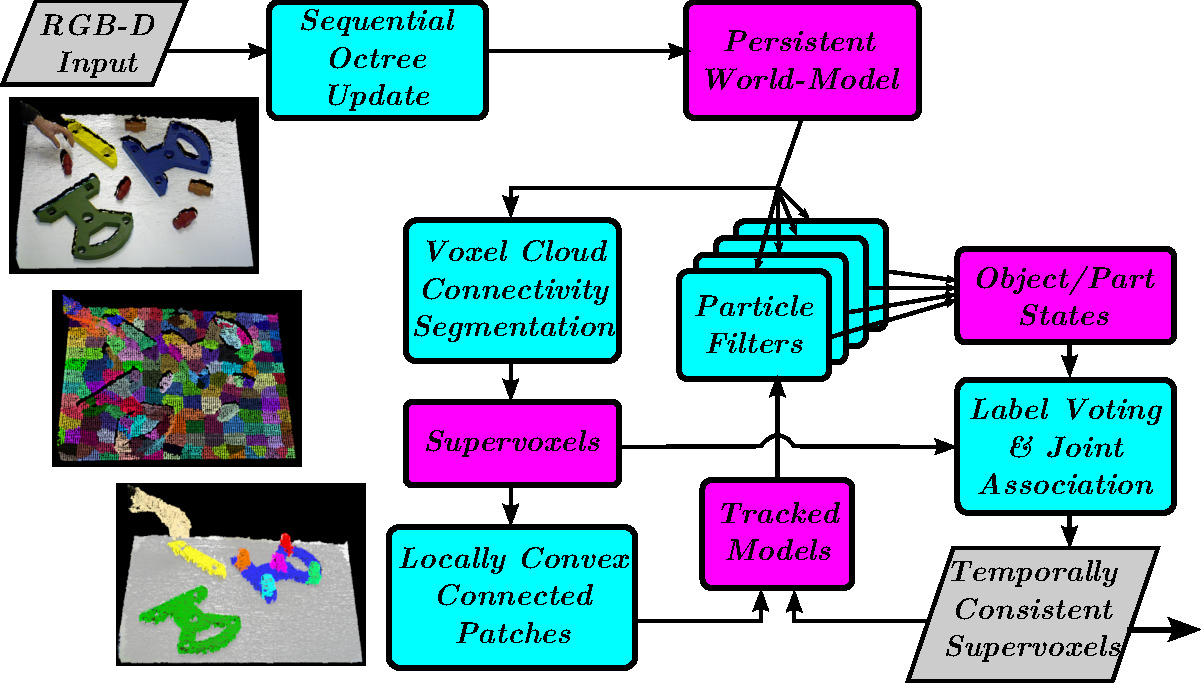
\includegraphics[width=\linewidth]{figures/Tracking/FlowChart.pdf}
  \caption[Algorithm Overview]{Overview of the algorithm for extracting temporally consistent supervoxels. The persistent world model, \gls{vccs}, \gls{lccp}, and particle filters function as presented in previous Chapters. The key addition is the label voting and joint association scheme which uses tracked states to associate supervoxels from frame to frame. The output of this is then fed back to the trackers to update their models. }
  \label{fig:AlgFlowChart}
\end{figure}
The first issue that must be addressed is the ``level'' at which targets should be tracked - the object or the supervoxel level (we shall not consider tracking at the voxel level since it is computationally infeasible with current hardware). As our goal is to associate supervoxels across time, we would like to track supervoxels directly. Unfortunately, this is generally not feasible due to the ``aperture problem'' seen in neural visual fields~\cite{MarrApertureProblem}. The aperture problem deals with the fact that local motion can only be estimated perpendicular to a contour that extends beyond its field of view~\cite{shimojo1989}. In other words, determining direction of motion in a local region (without considering global features) is generally not possible - as illustrated in Figure \ref{fig:Aperture}. This means that in order to estimate motion of supervoxels, we must extend the field of view considered significantly beyond the size of the supervoxel itself; in fact, our aperture must contain the borders of the moving object in question, otherwise pairwise association of supervoxels is generally indeterminate. 

\begin{figure}[!t]
  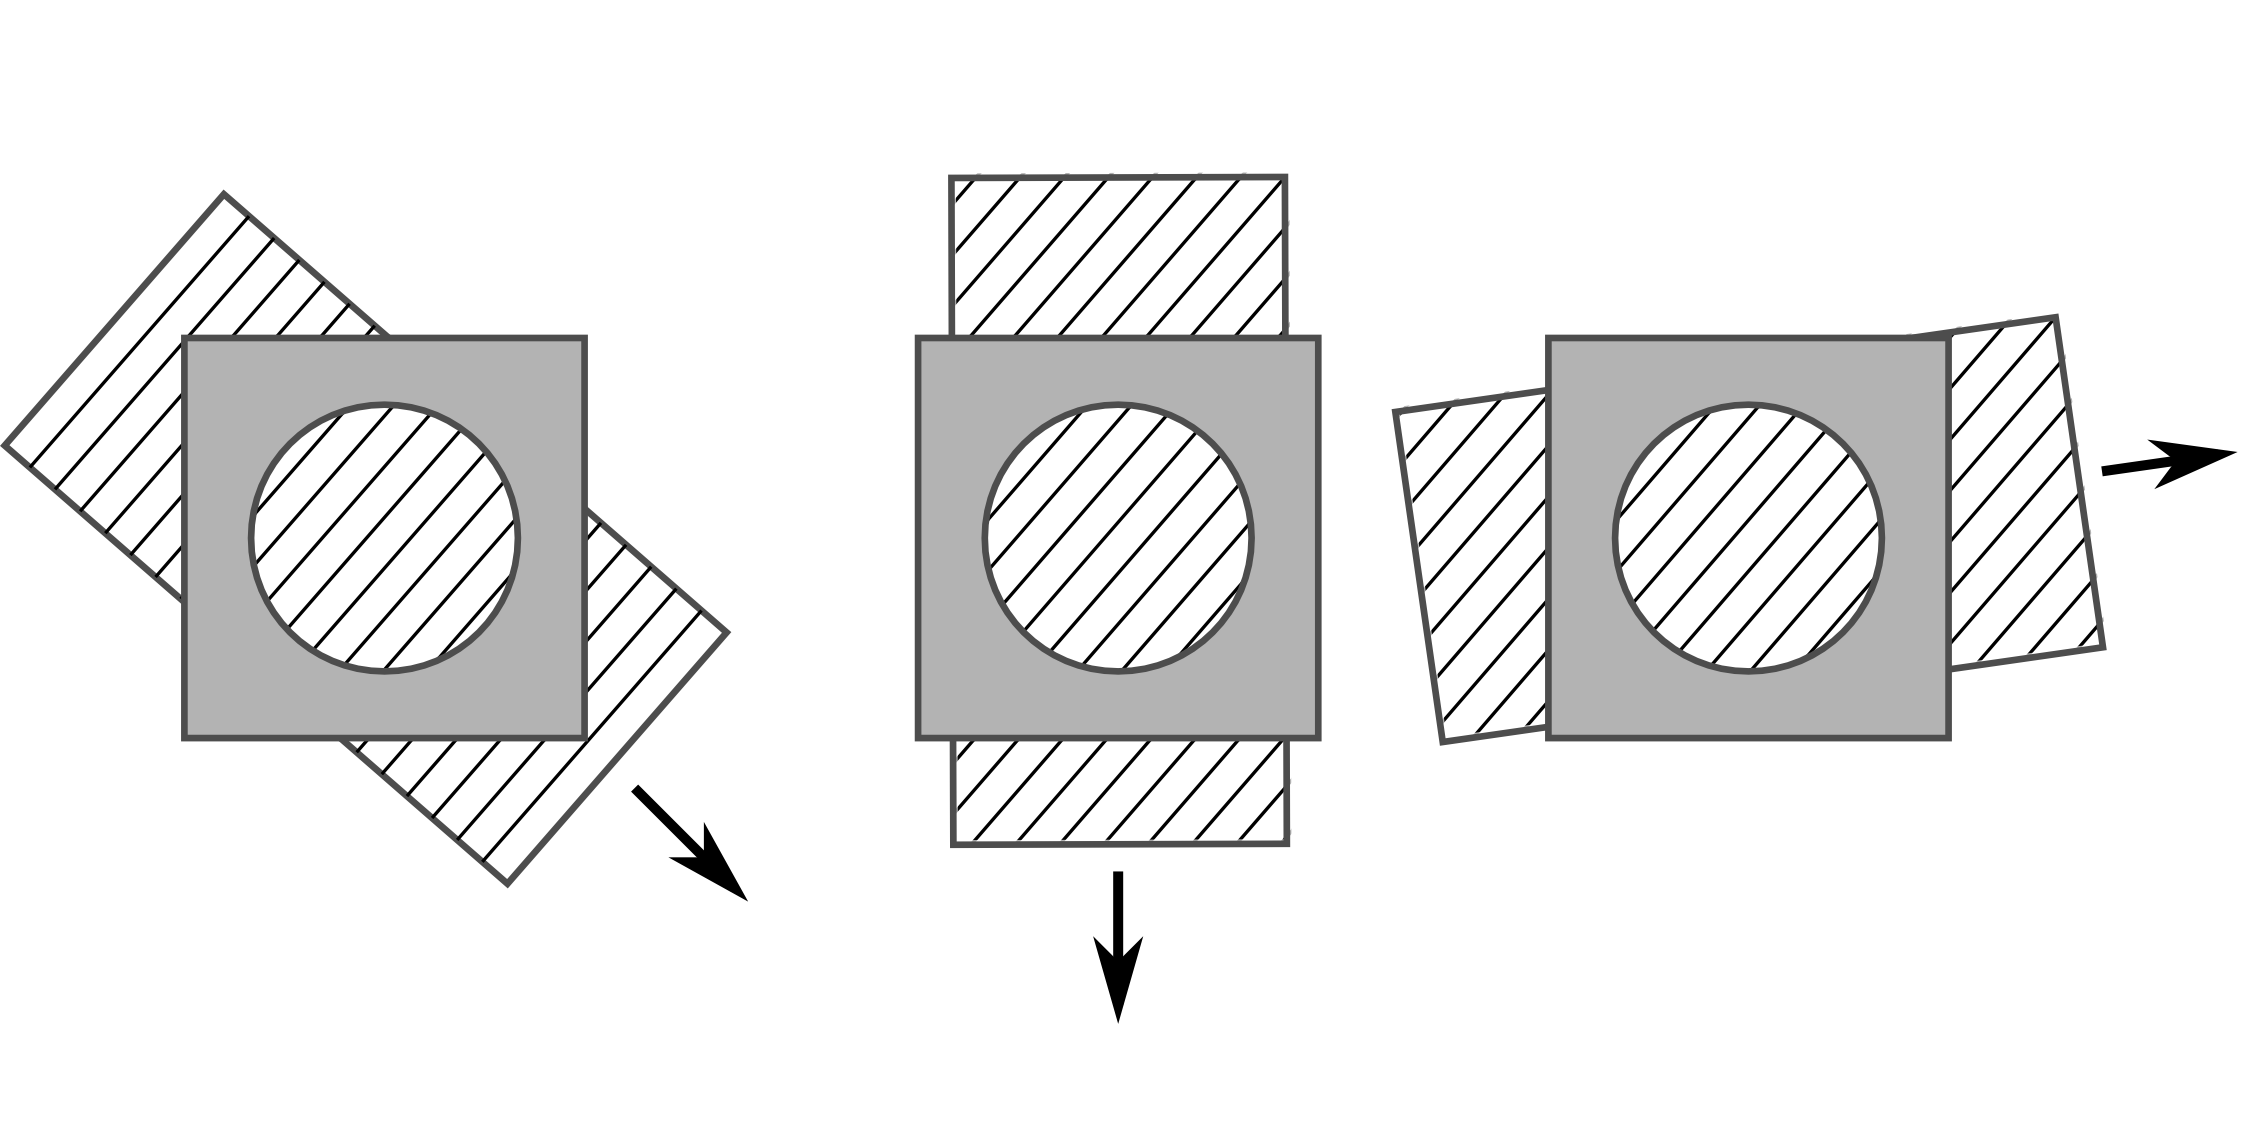
\includegraphics[width=\linewidth]{figures/Tracking/Aperture.png}
  \caption[The Aperture Problem]{The ``Aperture Problem'' - Three patterns moving in three different directions all produce the same perceived stimulus when viewed through a small aperture. In order to correctly resolve direction of motion a wider field of view is needed. Adapted from \cite{kandel2000principles}.}
  \label{fig:Aperture}
\end{figure}

Thud we must track higher level groupings - groupings that extend at least to a contour which provides a reference boundary for disambiguating motion. A natural way of doing this is to use the LCCP segmentation presented in Chapter \ref{Chap:WorldModel}, as it will expand regions up to concave boundaries. Using concave connections as references is surprisingly powerful, as it generally will differentiate objects, as well as parts of objects which can move independently (consider the case of joints in the human body). As such, we adopt a simple scheme for grouping supervoxels into tracked models; we perform LCCP segmentation on the first frame, and assign each observed segment to an independent tracker.

\section{Bank of Parallel Particle Filters}
Tracking of the segmented objects or parts is accomplished using a bank of the correspondence-based particle filters from the previous Chapter. We select a measurement model based on the voxels and supervoxels produced using the persistent world-model scheme discussed in Chapter~\ref{Chap:WorldModel}. The model measures distance in a feature space of spatial distance, normals, and color. Weights of predicted states $\mathbf{x}^j_t = [d_x, d_y, d_z, \gamma, \beta, \alpha]$ are measured as in the previous Chapter by associating transformed model voxels to the observed voxels nearest in space. Particles are then weighted by measuring total distance in feature space, just as in Equation \ref{eqn:distance}.

\section{Association by Joint Label Optimization}
Since our goal is extract full segmentations, rather than just object states, we must actively associate observed supervoxels (and therefore, voxels) with tracked results. This can be considered as an additional step beyond the tracking of the previous Chapter, which used observations to test how well a particle prediction matched reality. We can begin by considering the trivial case of tracking a single object. In this case we can extract a segmentation by establishing a small search radius $R_assoc$ around each tracked model result point (giving us an ``association volume'' around each point). If we simply assign each observed voxel falling within this volume to the tracked model, we can easily achieve a rough segmentation. Furthermore, we can determine which supervoxels belong to the object (and which belong to the unlabeled set) using a majority-voting scheme. This gives us a ``foreground segmentation'' method, which segments out the tracked object as foreground. 

Extending this to multiple objects, observe that the difficulty now lies in resolving associations of voxels which lie within the association volume of two or more tracked results. Fortunately, most voxels will only fall within the volume of a single object's tracked model, leaving us with only having to resolve associations along interacting object boundaries. As such, we begin by composing a list of all supervoxels which are under competition, that is, have voxels falling within the association volumes of more than one label. We can then count the number of voxels associated to each object, and normalize to give us an a-priori categorical distribution ${P}(L(p) = k | V )$ which maps labeling of supervoxels $p \in P$  to objects $k \in K$ given voxel associations $V$.  

%More formally, for a set of object labels $L$, supervoxels $S$, and voxels $V$ in an image frame, we first use the association volume to assign labels to voxels. This results in having a set of associated labels for each voxel in $V$, where 
\begin{figure}[tb]
  \centering
  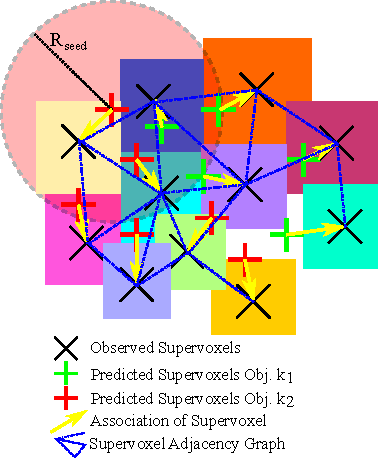
\includegraphics[scale=1.0]{figures/IROS2013/Association.pdf}
  \caption[Supervoxel Association]{Association of observed supervoxels with predicted model supervoxels using smoothing term which considers neighbor labels.}
  \label{fig:Association}
\end{figure}

Now that we have priors for object labelings, we adopt a Monte Carlo approach, similar to \cite{EnergyBasedMultiModel}, to sample from the set of possible label associations and determine a global association which best aligns tracked object predictions to observed supervoxels. To generate realizations (sets of label assignments), we use a weighted sampling strategy which considers the priors, as well as a distance term. This gives us a likelihood of assigning object label $k$ to supervoxel $p$ given distance from the object centroid $C_k$ and the voxel associations:
\begin{equation}
 \label{eqn:WeightSampling}
 \mathcal{L}(L(p)=k | C_k, V). %{P}(L(p) = k | V ) \frac{1}{C_k}.
\end{equation}

To compute a score for each realization, we use the global energy function given in~(\ref{eqn:Energy}). Each global label association $\mathcal{A}$ consists of a set of associations $\{a_1 \dots a_n\}$ which assign object labels $k$ to the set of observed supervoxels $\{p_1 \dots p_n\}$. The first summation term, $ \sum_{p}{\|p^*_k - p\|} $, measures error in feature space between the observed supervoxel and the supervoxel of the stratum in its associated object $p^*_k$. 

\begin{equation}
\label{eqn:Energy}
{E}_\mathcal{A} = \left( \sum_{p}{\|p^*_k - p\|} + \lambda \sum_{(p,p')\in \mathcal{N} }\delta(L(p) \not= L(p')) \right) \prod_{a\in\mathcal{A}}{\Delta_k}
\end{equation}

The second summation is a smoothing term which considers the adjacency graph of observed supervoxels. For every observed supervoxel, we compare its assigned labeling $L(p)$ to the label of all supervoxels $p'$ which lie within its adjacency neighborhood $\mathcal{N}$. We adopt the Potts model as in \cite{Boykov2001}, where $\delta(\dot)$ is 1 if the specified condition holds, and 0 otherwise, and $\lambda$ is a weighting coefficient which controls the importance given to spatial smoothness of labels.

Finally, the multiplicative term $\prod_{a\in\mathcal{A}}{\Delta_k}$ controls for the expansion or contraction of objects through the number of observed voxels associated with them. $\Delta_k$ penalizes for changes in volume by increasing the energy for deviations from unity in the ratio of observed voxels assigned to an object $\hat{N}_k$ with the number in the object model itself $\hat{N}_k$, that is

\begin{equation}
\label{eqn:DeltaSVs}
\Delta_k = \left\{ 
  \begin{array}{l l}
    {\hat{N}_k}/{N_k} & \quad \text{if ${\hat{N}_k} \geq {{N}_k}$ }\\
    2 - {\hat{N}_k}/{N_k} & \quad \text{if $\hat{N}_k < {N}_k$}~. 
  \end{array} \right.  
\end{equation}

Once we have arrived at a stable minimum energy score, we extract the resulting association of observed supervoxels to predicted results, and use them to update the tracked models.

\section{Alignment and Update of Models}
The joint energy minimization results in a global association $\mathcal{A}$ which assigns observed supervoxels to tracked objects. In order to use this to update the object models, we must align it to the internal representation stored by the particle filter. We begin at the inverse of the predicted state, and then use an iterative closest point \cite{ICPChetverikov} procedure to refine the transform such that the set of observed supervoxels best aligns with the model. We then update the model with the new observations by inserting the new supervoxels into the model. 

As a final step, we use the refined transform to update the states of the particles. To do this, we shift each particle $x_i$ towards the refined state $\hat{x}$, weighting the importance given to the refined state by a constant factor $\epsilon$

\begin{equation}
\label{eqn:PFUpdate}
x'_{i \in L} = (1-\epsilon) x_i + \epsilon \hat{x}~.
\end{equation}

For this work, we found that an $\epsilon$ of $0.5$ effectively removes noise (jitter) introduced by the replacement of the tracked model. Additionally, we correct the internal motion model ($\{v_x, v_y, v_z\}$) of the particle filters to correspond to the new updated state.

\section{Experimental Results}
As a demonstration of the method, in this Section we provide results from two successful applications. Both applications use the Cranfield scenario \cite{collins1984development} presented in the previous Chapter. Figure~\ref{fig:Trajectories} shows the results of tracking and segmentation on one assembly of the benchmark. It can be seen that the algorithm is able to successfully extract full segmentation of the video, as seen by the tracks and the segmented pieces.

\begin{figure*}[!ht]
  \centering
  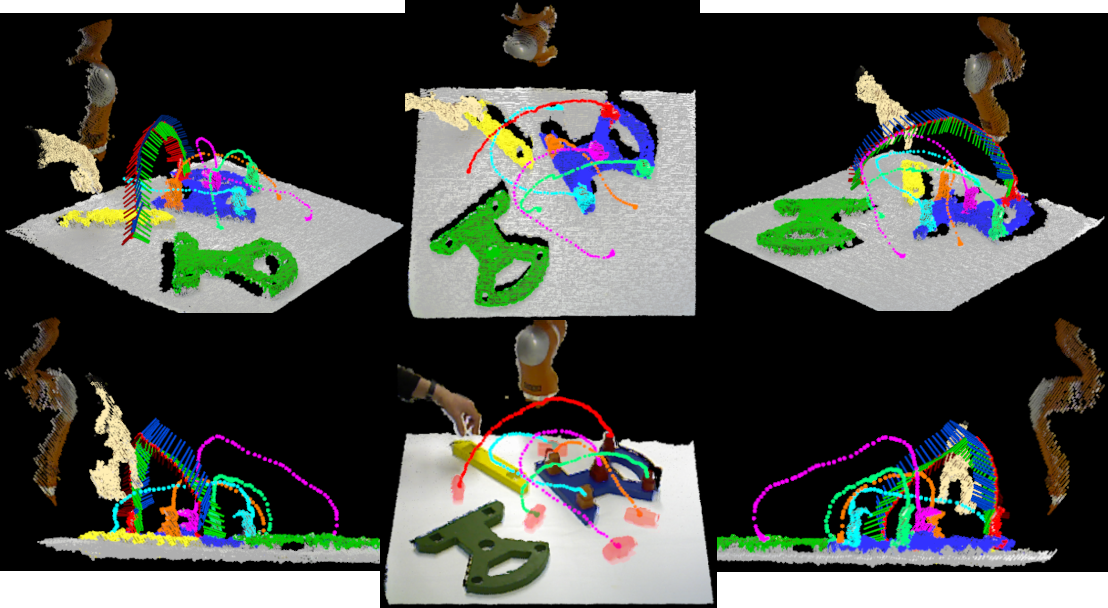
\includegraphics[width=\linewidth]{figures/IROS2013/TrajectoriesNew.pdf}
  \caption[Cranfield Tracking Results]{Result of tracking and segmentation on Cranfield scenario from different views. Here the tracks are shown as dots of the color of the tracked label for each timestep. Initial locations of the pegs are shown in the middle bottom frame as semi-transparent masks. Calculated orientation is shown for the red peg with a set of axes every second time-step; these axes show pose in a frame relative to the start. }
  \label{fig:Trajectories}
\end{figure*}

%%%%%%%%%%%%%%%%%%%%%%%%%%%%%%%%%%%%
\subsection{Imitation of Trajectories for Robot Manipulation}
\begin{figure}[!tb]
  \centering
  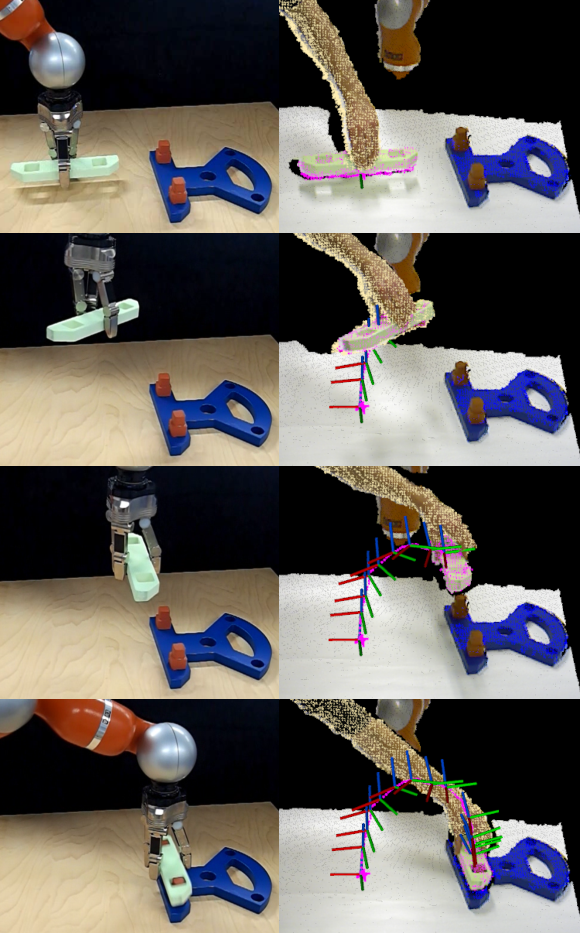
\includegraphics[scale=0.84]{figures/IROS2013/RobotImitation.pdf}
  \caption[Trajectory Imitation]{Kuka LWR arm imitating trajectory and pose learned from tracked human demonstration.}
  \label{fig:Imitation}
\end{figure}
The standard way of teaching robots to perform human-like actions is imitation learning, also called programming by demonstration \cite{Billard2008,Argall2009}. There are several ways to demonstrate movements: 1) recording movements in joint-space (joint angles) or target-space (Cartesian space) by ways of a motion capture device (requires putting markers on human body), 2) using kinaesthetic guidance (guiding a robot's movements by a human hand), or 3) via teleoperation (controlling a robot via joystick). The only way to obtain motion trajectories from human observation in a "non-invasive" procedure is by using stereo vision \cite{Hecht2009}, however, usually it is model based. The tracking algorithm we have presented here can be used as an alternative method to obtain motion trajectories (in Cartesian space) in a model-free way. 

To demonstrate this, we applied our tracking algorithm to obtain human motion trajectories in Cartesian space including orientation of manipulated object (in total six DoFs). We tested it using a recording of the Cranfield scenario where, first, we let a human demonstrate the action and then reproduced it using a KUKA Light Weight Robot (LWR) arm \cite{kuka}. Specifically, here we imitate a human putting the separator block on the pegs. To generate trajectories for the robot from human demonstrations, we used a modified version of Dynamic Movement Primitives \cite{Ijspeert2002,Ijspeert2013} (DMP) and learning method as described in \cite{Kulvicius2012}. We used Cartesian impedance control and, thus, generated six DMPs (three for motion of the end-effector in Cartesian space and three for orientation of the hand) based on trajectories obtained from the tracking algorithm. Here we used 100 equally spaced kernels with width $\sigma=0.05$ for each dimension (for more details please refer to \cite{Kulvicius2012}).
 As demonstrated in Figure~\ref{fig:Imitation} and the supplementary video, trajectories obtained by the proposed tracking algorithm are sufficiently accurate to allow reproduction of the human motion. We should emphasize that the key advantage here over the tracking from the previous Chapter is that we can track and segment out the human arm - something not possible with a rigid-model approach.

%%%%%%%%%%%%%%%%%%%%%%%%%%%%%%%%%%%%

\subsection{Semantic Summaries of Actions}
A fundamental task for intelligent autonomous robots is the problem of encoding long chain manipulations in a generic way, for use in tasks such as learning and recognition. As a demonstration of the usefulness of the proposed tracking framework, we use a recently introduced novel Semantic Event Chain (SEC) approach \cite{Aksoy11} which converts each segmented scene to a graph: nodes represent segment (i.e. object) centers and edges indicate whether two objects touch each other or not. By using an exact graph matching technique the SEC framework discretizes the entire graph sequence into decisive main graphs. A new main graph is identified whenever a new node or edge is formed or an existing edge or node is deleted. Thus, each main graph represents a “key frame” in the manipulation sequence. Figure~\ref{fig:SECGraphs} shows a few detected sample key frames from the long Cranfield action. While the complete action has in total 1453 frames, the SEC representation reduces it to just 12 key frames, each of which represents a topological change in the scene.

\begin{figure*}[ht!]
  \centering
  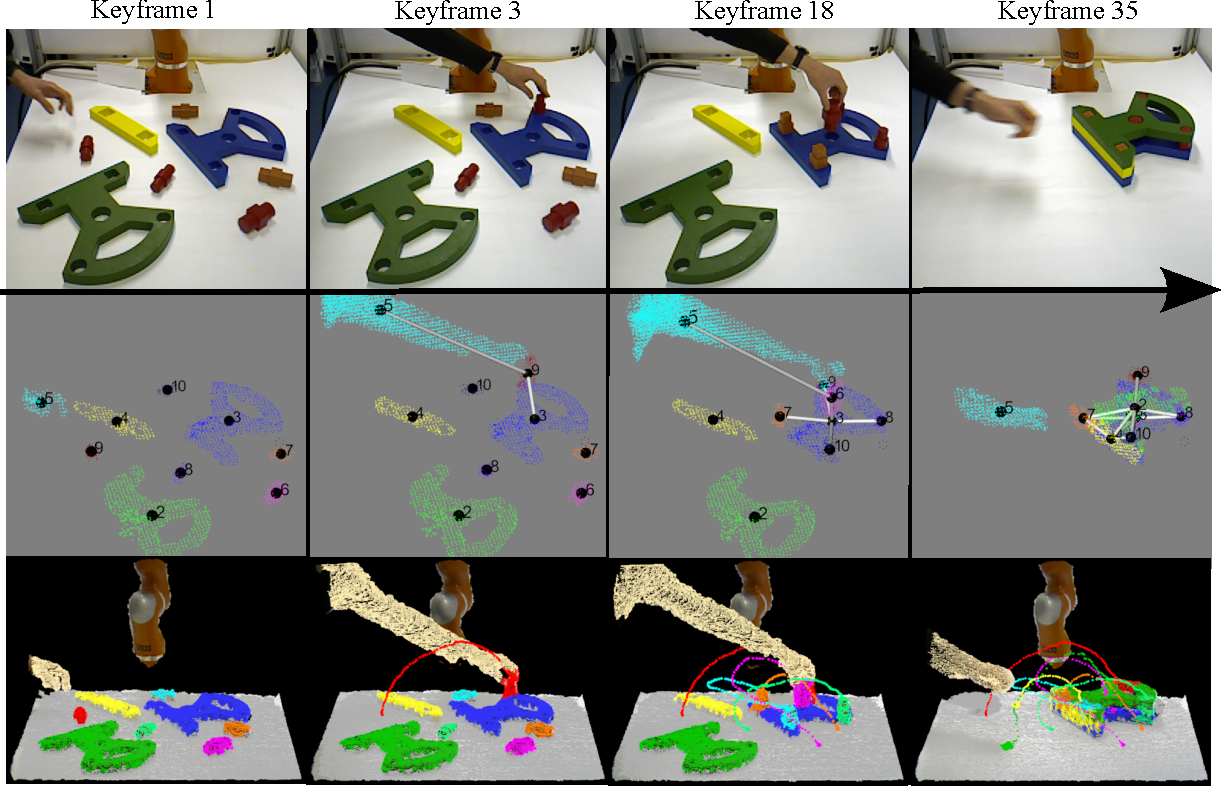
\includegraphics[width=\linewidth]{figures/IROS2013/SECKF.pdf}
  \caption[Cranfield Key Frames]{A few example key frames extracted from the long Cranfield action. Numbered nodes represent interacting objects, while edges show touching relations between objects. Each keyframe represents a topological change in the scene - here we show 4 of the 12 keyframes.}
  \label{fig:SECGraphs}
\end{figure*}

\section{Discussion}
In this Chapter we presented a method which extracts full scene segmentation from the model tracker we presented in the previous Chapter. The method uses a global energy functional to enforce smoothness and temporal continuity on the segmentations. Additionally, we feed segmentation results back into the tracked models, updating them so that they can deform and/or accumulate different view points. This allows us to extract a full video segmentation from our tracked states.

There are many advantages to the method presented in this Chapter over the model tracker - it can track deforming objects, there is no need to know object models a-priori, tracked objects can be easily re-initialized using LCCP segmentation, there is no need to compute initial poses, and finally, we can extract action semantics without needing to know what objects are present. As this approach is completely free of trained models or strict object boundaries, it opens up many avenues of future research. In particular, of especial interest is that it allows bootstrapping of learning - we can attempt to build systems which learn to understand scenes purely from observation, without any human input or teaching.